\section{Specific Requirements}\label{sec:spec_req}

Here we include more details on all aspects in Section 2 if they
can be useful for the development team. 

\subsection{External Interface Requirements}
\subsubsection{User Interfaces}

The application is designed to allow the customer to make a reservation for a certain hour
or to register in the current queue of a supermarket. The first time the user opens the app,
they are prompted to register for an account: they have to provide their mobile phone number
(Fig. \ref{fig:mockup-welcome}), then they'll receive an SMS with a confirmation code
(Fig. \ref{fig:mockup-login}) to insert.
If the code inserted is the one sent to the phone number inserted in the first screen, the
account creation is successful.

If the registration is successful, the user can immediately see a map (Fig \ref{fig:select-store})
with stores nearby their location (they might have to allow the app do receive their location through
the OS API), otherwise they can manually search stores by typing an address.
Stores are also listed by distance and queue length.

Upon selecting a store (Fig. \ref{fig:store-details}), the current number of people in queue is shown to the user,
as well as the estimated waiting time in queue. They can choose to enter the queue as soon as
possible, or to pick an available time slot.

If they choose to pick a time slot, they are shown a list of time slots sorted by day (Fig. \ref{fig:select-timeslot}).
Upon confirmation, the user receive a receipt (Fig. \ref{fig:receipt}) with the date and time of their reservation,
and a QR code that they'll need to show when they present themselves at the store.

Should the customer queue for the first available time slot, then they will receive a similar receipt (Fig. \ref{fig:queue-ticket}),
that has a countdown of the time remaining in queue before their visit.

\begin{figure}[h]
    \caption{Mock-up of the Application User Interface}
    \subfloat[Welcome Screen]{
        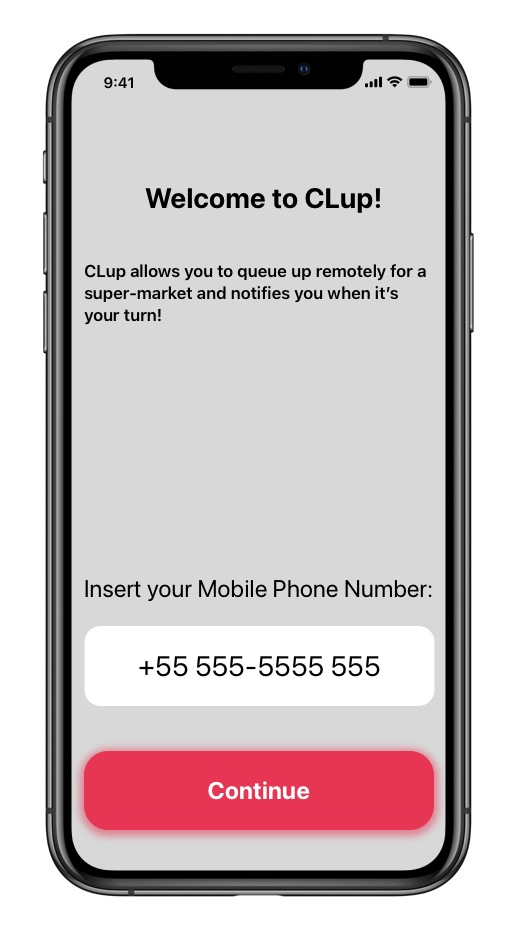
\includegraphics[width=0.25\textwidth]{images/mockup/welcome-screen.png}
        \label{fig:mockup-welcome}
    }
    \subfloat[Confirm Login]{
        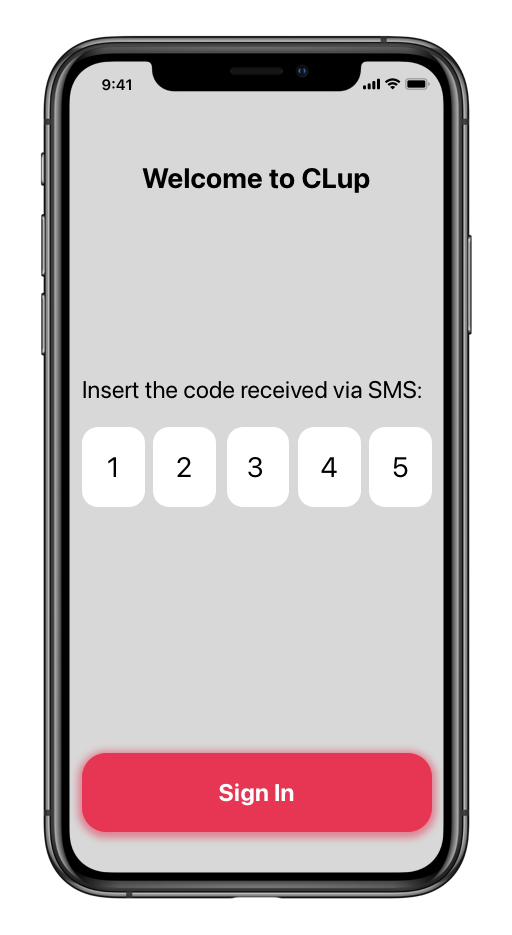
\includegraphics[width=0.25\textwidth]{images/mockup/confirm-login.png}
        \label{fig:mockup-login}
    }
    \subfloat[Select Store]{
        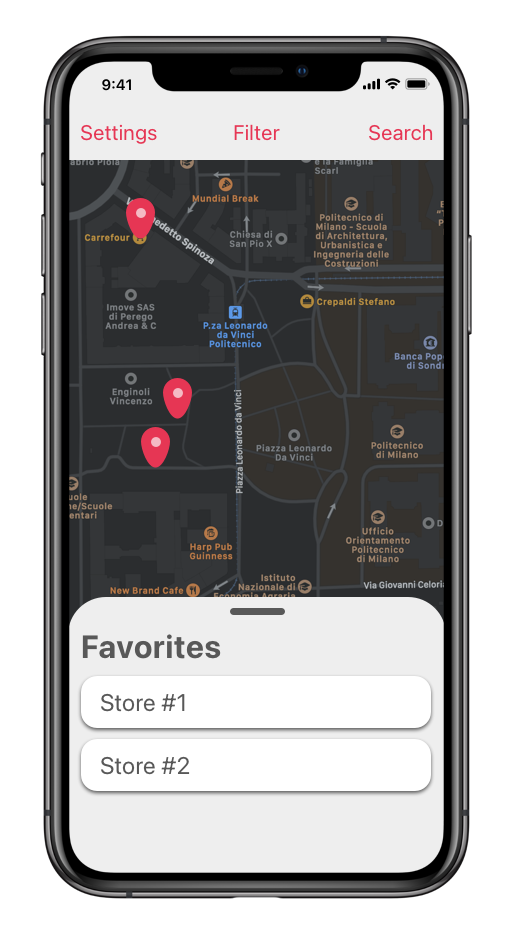
\includegraphics[width=0.25\textwidth]{images/mockup/map-select.png}
        \label{fig:select-store}
    }
    \subfloat[Store Details]{
        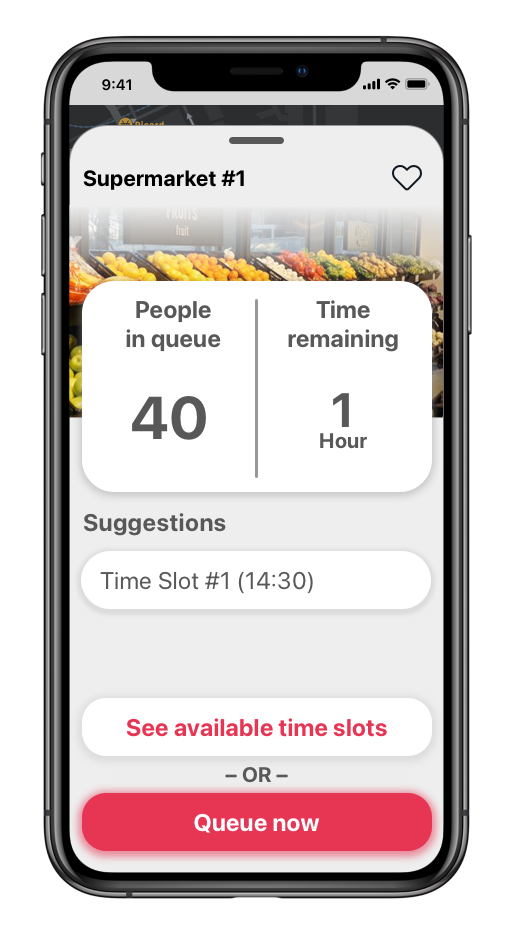
\includegraphics[width=0.25\textwidth]{images/mockup/store-detail.png}
        \label{fig:store-details}
    }
    \newline
    \subfloat[Select Timeslot]{
        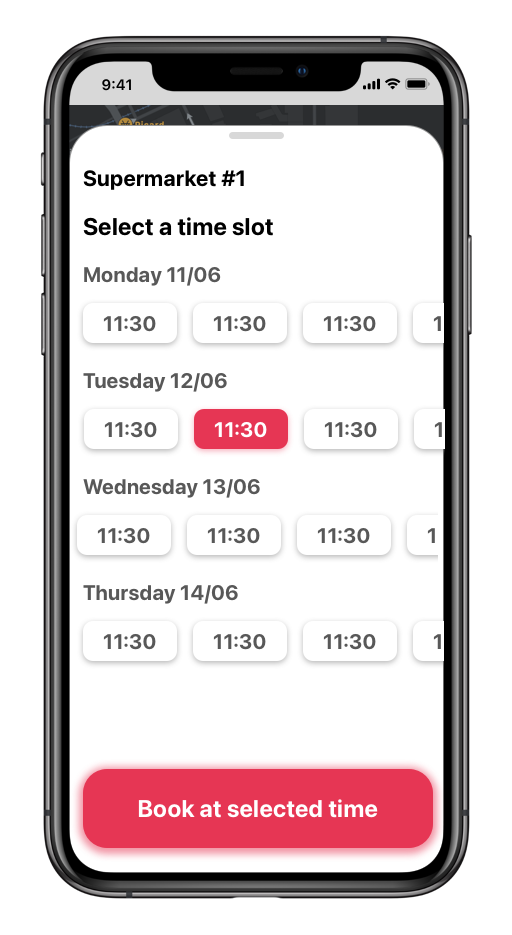
\includegraphics[width=0.25\textwidth]{images/mockup/time-slots.png}
        \label{fig:select-timeslot}
    }
    \subfloat[Reservation Receipt]{
        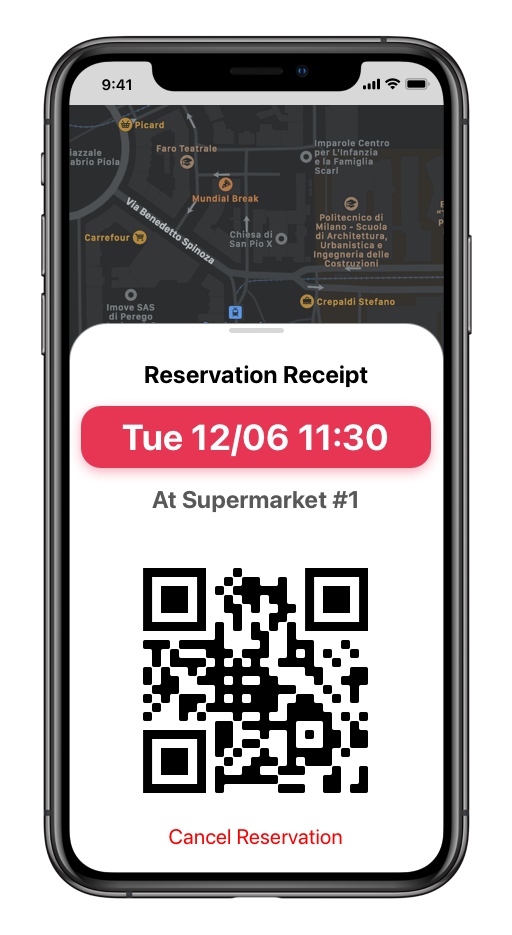
\includegraphics[width=0.25\textwidth]{images/mockup/receipt.png}
        \label{fig:receipt}
    }
    \subfloat[Queue Ticket]{
        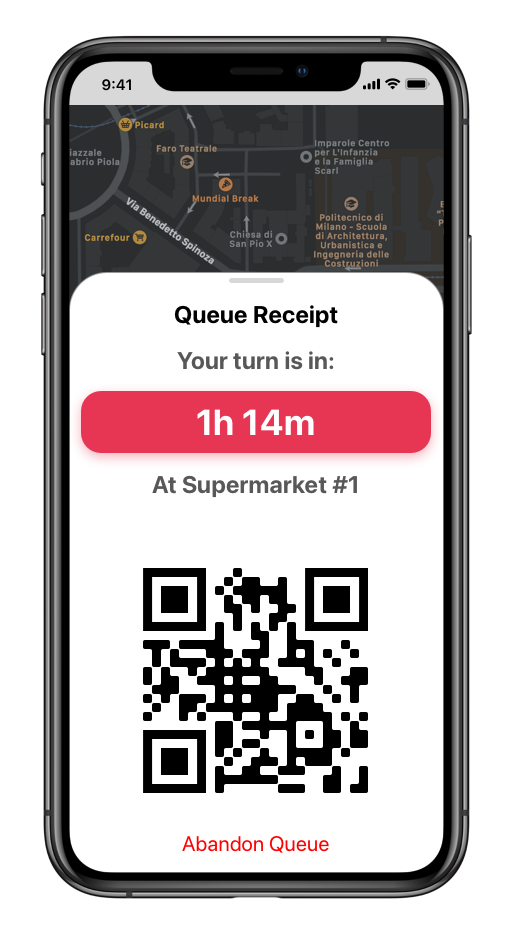
\includegraphics[width=0.25\textwidth]{images/mockup/queue-ticket.png}
        \label{fig:queue-ticket}
    }
\end{figure}


\subsubsection{Hardware Interfaces}

To account for Customers without an Internet-connected device,
an interactive totem (Fig. \ref{fig:totem}) with a touchscreen display should be made available at each store entrance.
The totem is connected to Internet or the store local network.
It mirrors the key features of the web application, but it doesn't require the customer to
authenticate. Customers may reserve a time-slot, or enter the queue, but they won't be able to
be notified of possible changes. The reservation receipt is printed and the customer must keep it until they're
admitted to the store, otherwise they won't be able to enter.
\begin{figure}[h]
    \centering
    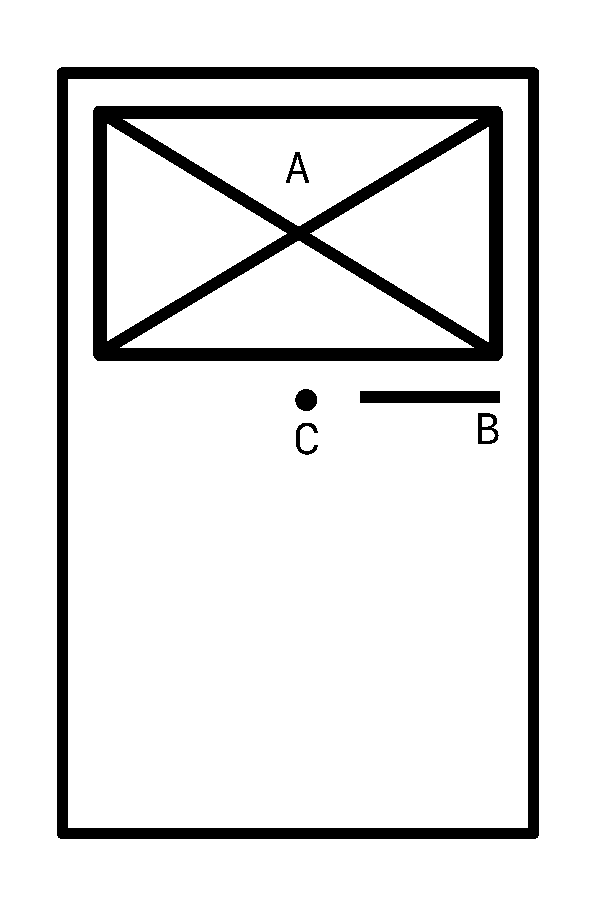
\includegraphics[width=0.25\textwidth]{images/totem.pdf}
    \caption{The totem interface: (A) is the touchscreen display,
    (B) is where the printed ticket is emitted, (C) is a proximity sensor that wakes the
    totem when a client is nearby.}
    \label{fig:totem}
\end{figure}

\subsubsection{Software Interfaces}
\subsubsection{Communication Interfaces}

\subsection{Functional Requirements}
Definition of use case diagrams, use cases and associated
sequence/activity diagrams, and mapping on requirements

\begin{enumerate}[label={[R\arabic*]}]
    % Users
    \item Allow a User to find Stores nearby a specified location.
    \item Allow a User to get in the virtual line.
    \item Allow a User to preview an estimate of the queue time.
    \item Allow a User to cancel their reservation.
    \item Allow a User to retrieve a scannable QR Code/Barcode that they must present in order to be granted access to a store.
    \item Allow a User to sign up for an Account after providing a mobile phone number.
    \item Allow a registered User to book a visit for themselves or for someone else to a specific store.

    % Store
    \item The System notifies the Users affected by delay.
    \item The System postpones Users visits in case of a delay.
    \item The System enforces the limits on the allowed number of concurrent Customers inside a store.
    \item The System does not admit Users that arrive earlier, even if the current number of Customers isn't maximum.
    \item The System grants a User access only after the User's time of reservation.
    \item The System invalidates a User's reservation if they do not show up during a certain time interval.
    \item The System reserves a certain number of the allowed quote of customers for a special category of Users.
    \item The system grants priority access to Users without a reservation that show up at the store and are pregnant women, elderly or with disabilities.
    
    % System Managers
    \item Allow System Managers to set a limit to the people allowed into the store at a time.
    \item Allow System Managers to not provide the physical ticket option.
    \item Allow System Managers to enable the functionality that allows customers to link their Account with Loyalty Program feature.
\end{enumerate}

\begin{center}
    \begin{tabular}{ |c||c|c| }
        \hline
        \textbf{Goal} & \textbf{Requirements} & \textbf{Assumptions} \\
        \hline
        G1 & R1, R2, R3, R4, R5, R6 & \\
        \hline
        G2 & R3, R7, R8, & \\
        \hline
        G3 & R5, R10 & \\
        \hline
        G4 & & \\
        \hline
        G5 & & \\
        \hline
    \end{tabular}
\end{center}




%----------------------------------------------------------------------------------------------------
%                                           USE CASES
%----------------------------------------------------------------------------------------------------

%LOGIN
\usecase
{Sign Up}
{Customer}
{The Customer has installed the application on their device.}
{
    \begin{enumerate}
        \item The Customer opens the application.
        \item The Customer may read Privacy Policy and the Terms of Service by clicking on the respective links. If they create an account, it's implied that they accept them.
        \item The Customer enters their mobile phone number and taps ``Continue''.
        \item The Customer enters the received code via SMS and taps ``Sign In''.
    \end{enumerate}
}
{The Customer is now logged-in and they may utilize the application.}
{
    \begin{itemize}
        \item The Customer inputs invalid data.
        \item The Customer doesn't fill the required data.
    \end{itemize}
}
{
    When an exception occurs, the user is informed by a human-readable message.
}


%Join Line
\usecase
{Join Line}
{Authenticated User}
{Authenticated User selects a Supermarket in the application}
{
        \begin{enumerate}
            \item The Authenticated User pushes the "Queue Now" button.
            \item The system provides the Queue Receipt with the generated QR code and the estimated time remaining.
        \end{enumerate}
}
{
    The customer is now in the queue waiting for their turn.
}
{
    \begin{itemize}
        \item There is a major delay in the store. 
        \item The time remaining to wait in the queue exeeds the opening hours of the store. 
    \end{itemize}
}
{
    When an exception occurs, the user has the possibility to remain in the queue or leave it. 
}


%Check Status
\usecase
{Check Status}
{Authenticated User}
{Authenticated User logs-in in the application}
{
        \begin{enumerate}
            \item The System provides the user a list of the supermarkets near him.
            \item The Authenticated User is able to see a preview of the number of people in queue and the estimated waiting time. 
            \item The user selects the desired store. 
            \item The user is now able to see full screen the waiting time and the number of people in queue (and possibly other stats on the store).  
        \end{enumerate}
}
{
    The Authenticated User gain the knowledge on the waiting times and the number of people in queue in the stores near him/her. 
}
{
    \begin{itemize}
        \item There are no open stores in the area. 
        \item There are no stores in the area. 
    \end{itemize}
}
{
    When an exception occurs the users is promted to check the application again later or change the search area. 
}




\subsection{Performance Requirements}
\subsection{Design Constraints}
\subsubsection{Standards Compliance}
\subsubsection{Hardware Limitations}
\subsubsection{Any Other Constraint}
\subsection{Software System Attributes}
\subsubsection{Reliability}
\subsubsection{Availability}
\subsubsection{Security}
\subsubsection{Maintainability}
\subsubsection{Portability}